\chapter{Generating Binomial Random variables}

\setcounter{problem}{1}
\section{Goal}

\begin{fullwidth}

The goal of this lab is to simulate a binomial distribution using repeated Bernoulli trials and then compare it against the theoretical binomial distribution. Please add new function {\tt rbinomial()} to the existing {\tt stats/stats.py} file so that we can continue to build our library. To draw the graphs in this exercise, create file {\tt stats/plot\_rbinomial.py}.

\section{Discussion}

\step First, define a function in file {\tt stats/stats.py} that performs $n$ Bernoulli trials with probability $p$ of success. It should return the number of successes out of $n$:

\begin{pyverbatim}
def binomial(n,p):
    "Sim with prob p, n bernoulli trials; return number of successes"
    ...
\end{pyverbatim}

The code is just a loop that goes around $n$ times and uses a variable from $U(0,1)$, using your {\tt runif01()} function, to check for success or failure. For example, my solution assumes failure if the uniform random variable is greater than $p$.
    
\step Next, in {\tt stats/plot\_rbinomial.py}, import your uniform random number generator library (which include your new {\tt binomial()} function) and set the seed of the random number generator. (Otherwise you will always get the same Bernoulli trials.) 

\begin{pyverbatim}
from stats import *

# other stuff we need:
import time
import matplotlib.pyplot as plt
import scipy.misc as misc

# I defined a function to hide implementation details
setseed( int(round(time.time() * 1000)) )
\end{pyverbatim}

In this case, we're using the current time in milliseconds as the random seed so that it is different every time you run the program. (remember this trick.)

\step Now that we can know how to get a binomial random variable, we can examine the binomial distribution.  All we have to do is grab a vector of, say, $SAMPLES$ binomial random values and the plot a histogram.  The density function at $k$ is just how many successes out of $SAMPLES$ there were ($k/SAMPLES$ probability).

Let me introduce you to something called a {\em list comprehension} in Python, which is a for loop that results in a list. It's also considered a {\em map} function ala {\em map-reduce}.  Get list $X$ as $SAMPLES$ binomial values with parameters $n=500$ and $p=0.4$. Do that by simply calling the {\tt binomial} function $N$ times.

\begin{pyverbatim}
X = [binomial(n,p) for t in range(SAMPLES)]
\end{pyverbatim}

\step Plot the histogram normalized (normed=1) and run it. (You'll need {\tt hist()}.) You should see a graph similar to the following:

\scalebox{.35}{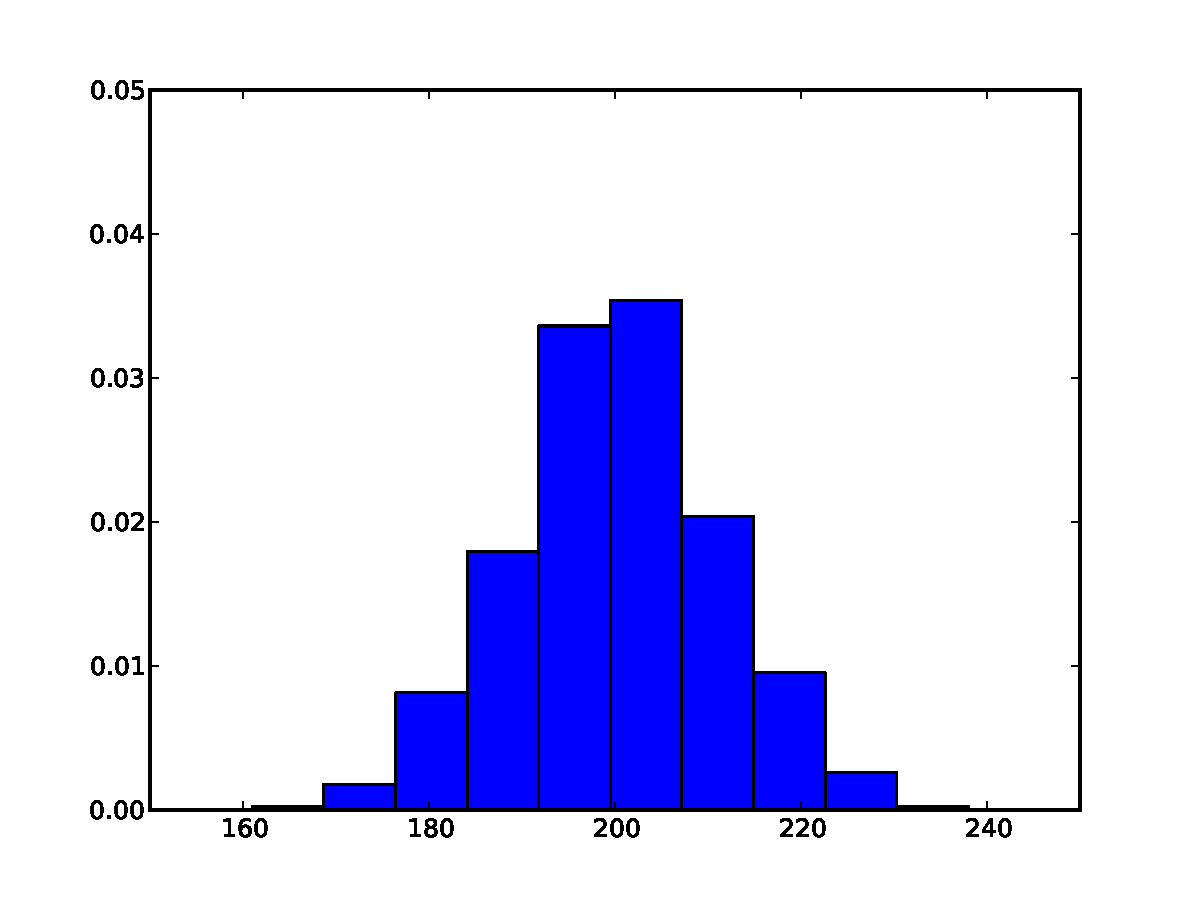
\includegraphics{figures/rbinomial-5000-4.pdf}}

\step We could use the built-in binomial mass function but let's define our own since it's easy:

\[\tag{Binomial mass function}
\binom{n}{k} p^k (1-p)^{n-k}
\]

\noindent That's the probability that there are $k$ successes in $n$ trials with probability $p$ of success. In {\tt stats/stats.py}, define a function like this:

\begin{pyverbatim}
def binom(n, k, p):
    """
    If we run n trials with p prob for each trial of success,
    what is probability of having k successes? You can use scipy.misc.comb() if you want.
    """
    ...
\end{pyverbatim}

\noindent You may use function {\tt scipy.misc.comb()} to compute $n \choose k$, but otherwise do the arithmetic yourself. (There is no loop in this function.)

\step To show the real distribution on top, we need to iterate $k$ across the range $0..n$ used in our empirical  simulation above.  Since this is a mass function not a smooth density function, we can use every fifth value in the range. Let's also add some text to describe the parameters.

\begin{pyverbatim}
Y = [binom(n, k, p) for k in range(0,n+1,5)]
plt.bar(range(0,n+1,5), Y, color='red', align='center', width=1)
plt.axis([150,250,0,.05]) # set the axes so that we get a close-up
plt.text(160,0.04, '$n = %d$' % N, fontsize=16)
plt.text(160,0.037, '$p = %f$' % P, fontsize=16)
plt.text(160,0.034, '$SAMPLES = %d$' % SAMPLES, fontsize=16)
\end{pyverbatim}

In this case I am not using 0..1 for the axes coordinates of the text; the default is the values of the graph itself. sometimes this is useful.

\step Run it and you should see something like the following:

\scalebox{.40}{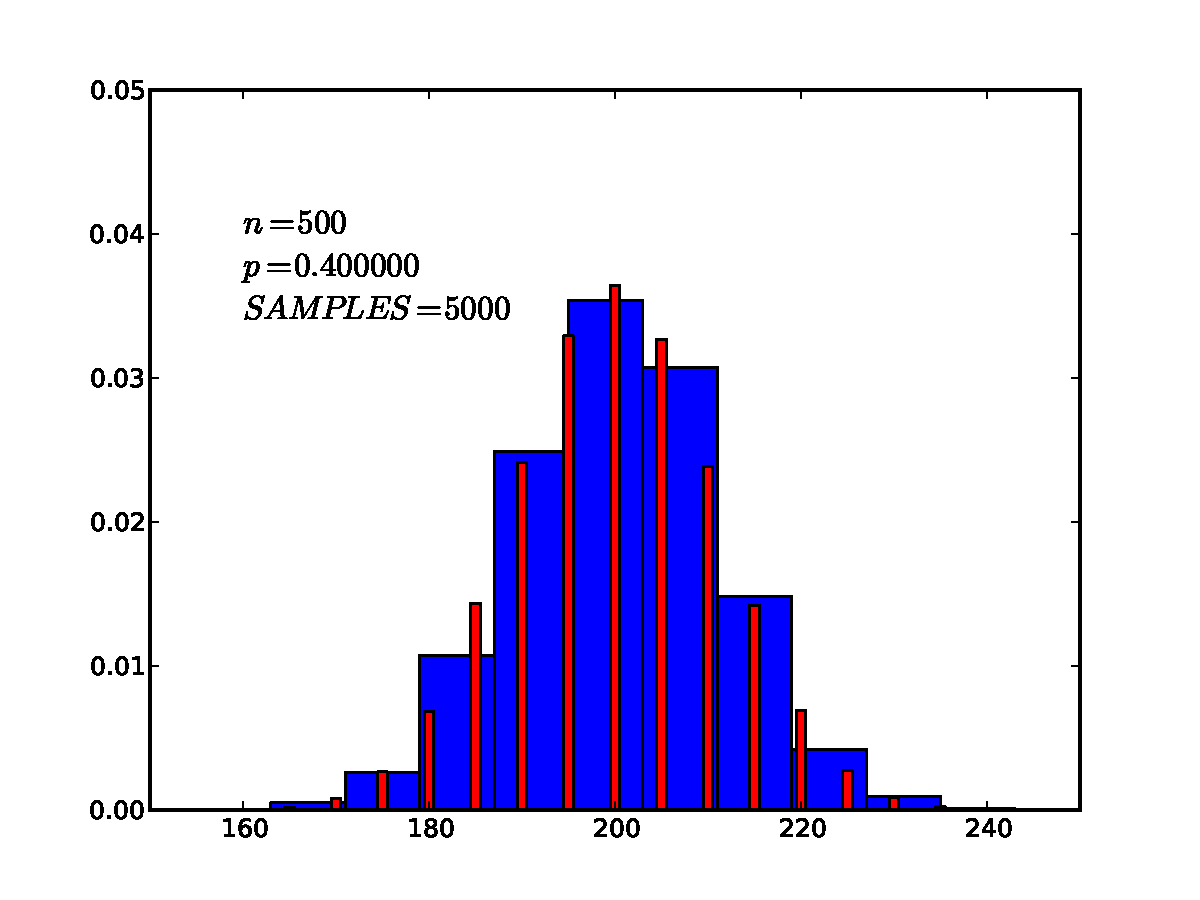
\includegraphics{figures/rbinomial-5000-4-fancy.pdf}}

Note that we use a bar chart for the binomial theoretical distribution and not a smooth graph because this is a mass function not a density function.

\begin{callout}{\bcplume}
{\bf Deliverables}. Make sure that {\tt stats/stats.py} has the new functions and that {\tt stats/plot\_rbinomial.py} ($n=500, p=0.4, SAMPLES=5000$) is correctly committed to your repository and pushed to github. 
\end{callout}

\end{fullwidth}
